% Created by tikzDevice version 0.12.6 on 2024-01-22 12:36:07
% !TEX encoding = UTF-8 Unicode
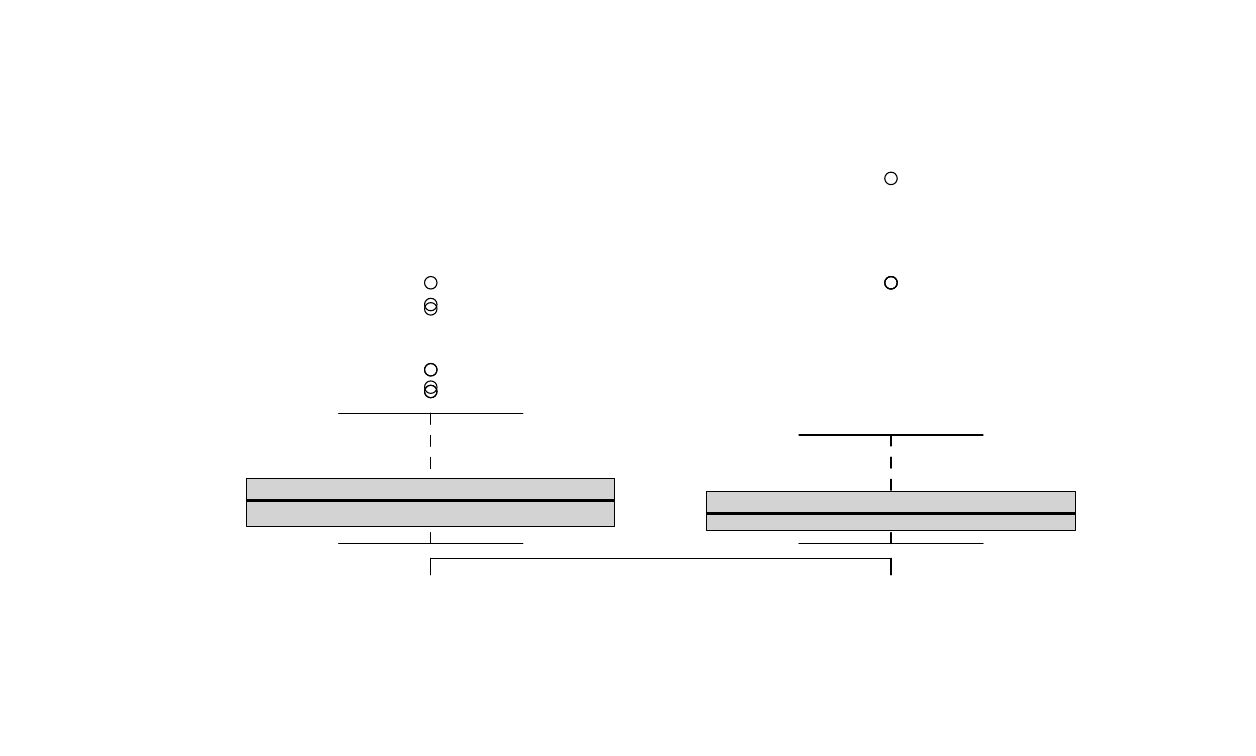
\begin{tikzpicture}[x=1pt,y=1pt]
\definecolor{fillColor}{RGB}{255,255,255}
\path[use as bounding box,fill=fillColor,fill opacity=0.00] (0,0) rectangle (433.62,252.94);
\begin{scope}
\path[clip] ( 49.20, 61.20) rectangle (408.42,203.75);
\definecolor{fillColor}{RGB}{211,211,211}

\path[fill=fillColor] ( 79.13, 72.76) --
	(212.18, 72.76) --
	(212.18, 90.05) --
	( 79.13, 90.05) --
	cycle;
\definecolor{drawColor}{RGB}{0,0,0}

\path[draw=drawColor,line width= 1.2pt,line join=round] ( 79.13, 82.19) -- (212.18, 82.19);

\path[draw=drawColor,line width= 0.4pt,dash pattern=on 4pt off 4pt ,line join=round,line cap=round] (145.66, 66.48) -- (145.66, 72.76);

\path[draw=drawColor,line width= 0.4pt,dash pattern=on 4pt off 4pt ,line join=round,line cap=round] (145.66,113.62) -- (145.66, 90.05);

\path[draw=drawColor,line width= 0.4pt,line join=round,line cap=round] (112.40, 66.48) -- (178.92, 66.48);

\path[draw=drawColor,line width= 0.4pt,line join=round,line cap=round] (112.40,113.62) -- (178.92,113.62);

\path[draw=drawColor,line width= 0.4pt,line join=round,line cap=round] ( 79.13, 72.76) --
	(212.18, 72.76) --
	(212.18, 90.05) --
	( 79.13, 90.05) --
	cycle;

\path[draw=drawColor,line width= 0.4pt,line join=round,line cap=round] (145.66,152.90) circle (  2.25);

\path[draw=drawColor,line width= 0.4pt,line join=round,line cap=round] (145.66,121.47) circle (  2.25);

\path[draw=drawColor,line width= 0.4pt,line join=round,line cap=round] (145.66,129.33) circle (  2.25);

\path[draw=drawColor,line width= 0.4pt,line join=round,line cap=round] (145.66,121.47) circle (  2.25);

\path[draw=drawColor,line width= 0.4pt,line join=round,line cap=round] (145.66,123.04) circle (  2.25);

\path[draw=drawColor,line width= 0.4pt,line join=round,line cap=round] (145.66,160.76) circle (  2.25);

\path[draw=drawColor,line width= 0.4pt,line join=round,line cap=round] (145.66,151.33) circle (  2.25);

\path[draw=drawColor,line width= 0.4pt,line join=round,line cap=round] (145.66,129.33) circle (  2.25);

\path[fill=fillColor] (245.44, 71.19) --
	(378.48, 71.19) --
	(378.48, 85.33) --
	(245.44, 85.33) --
	cycle;

\path[draw=drawColor,line width= 1.2pt,line join=round] (245.44, 77.48) -- (378.48, 77.48);

\path[draw=drawColor,line width= 0.4pt,dash pattern=on 4pt off 4pt ,line join=round,line cap=round] (311.96, 66.48) -- (311.96, 71.19);

\path[draw=drawColor,line width= 0.4pt,dash pattern=on 4pt off 4pt ,line join=round,line cap=round] (311.96,105.76) -- (311.96, 85.33);

\path[draw=drawColor,line width= 0.4pt,line join=round,line cap=round] (278.70, 66.48) -- (345.22, 66.48);

\path[draw=drawColor,line width= 0.4pt,line join=round,line cap=round] (278.70,105.76) -- (345.22,105.76);

\path[draw=drawColor,line width= 0.4pt,line join=round,line cap=round] (245.44, 71.19) --
	(378.48, 71.19) --
	(378.48, 85.33) --
	(245.44, 85.33) --
	cycle;

\path[draw=drawColor,line width= 0.4pt,line join=round,line cap=round] (311.96,160.76) circle (  2.25);

\path[draw=drawColor,line width= 0.4pt,line join=round,line cap=round] (311.96,160.76) circle (  2.25);

\path[draw=drawColor,line width= 0.4pt,line join=round,line cap=round] (311.96,198.47) circle (  2.25);

\path[draw=drawColor,line width= 0.4pt,line join=round,line cap=round] (311.96,160.76) circle (  2.25);
\end{scope}
\begin{scope}
\path[clip] (  0.00,  0.00) rectangle (433.62,252.94);
\definecolor{drawColor}{RGB}{0,0,0}

\path[draw=drawColor,line width= 0.4pt,line join=round,line cap=round] (145.66, 61.20) -- (311.96, 61.20);

\path[draw=drawColor,line width= 0.4pt,line join=round,line cap=round] (145.66, 61.20) -- (145.66, 55.20);

\path[draw=drawColor,line width= 0.4pt,line join=round,line cap=round] (311.96, 61.20) -- (311.96, 55.20);
\end{scope}
\end{tikzpicture}
